\documentclass[11pt]{article}
\usepackage{geometry}                % See geometry.pdf to learn the layout options. There are lots.
\geometry{letterpaper}                   % ... or a4paper or a5paper or ...
%\geometry{landscape}                % Activate for for rotated page geometry
%\usepackage[parfill]{parskip}    % Activate to begin paragraphs with an empty line rather than an indent
\usepackage{graphicx}
\usepackage{amssymb}
\usepackage{pgf}
%\usepackage{epstopdf}
\usepackage{url}
\DeclareGraphicsRule{.tif}{png}{.png}{`convert #1 `dirname #1`/`basename #1 .tif`.png}
\setcounter{secnumdepth}{7}
\setcounter{tocdepth}{7}


\title{XMLPipeDB: A Reusable Tool Chain for Building Relational Databases from XML Sources}
\author{
John David N. Dionisio \and
Joey Barrett \and
Joe Boyle \and
Adam Carasso \and
David Hoffman \and
Babak Naffas \and
Jeffrey Nicholas \and
Roberto Ruiz \and
Scott Spicer \and
Kam D. Dahlquist\\
\\
Loyola Marymount University
}
%\date{}                                           % Activate to display a given date or no date

\begin{document}

\maketitle

\abstract{
The abstract should be 150 to 200 words long and should consist of short, direct, and complete sentences. It should state the objectives of the work, summarize the results, and give the principal conclusions and recommendations. It should indicate clearly whether the focus is on theoretical developments or on practical questions and whether subject or method is emphasized. The title need not be repeated. Work planned but not done should not be described in the abstract.
}

\section{Introduction}
We started out with a problem: build a tool that will take an XML file from a gene information storage giant, like Uniprot and convert it to a GenMAPP file. At first this seemed to be an easy problem. Using tools like Hyperjaxb and Hibernate, we would be able to easily build a simple tool to accomplish this task. After building that simple tool, we found that things were not so straight forward. So, we broke up the task into several modules and went to work. This paper describes the motivations behind our original goal, the solution we finally agreed on, and how that solution fits together. Also, we will explore how our solution not only solves the problem we originally set out to solve for the bioinfomatics community, but solves some other problems for the general computing and computer science communities.


\section{Background and Motivation}
With the introduction of DNA micro arrays.  the need for tools to aid in the processing of large amounts of Bioinformatic data are needed.  Data can now be collected in larger sizes than ever before and would be nearly impossible to analyze by hand.  GenMapp is a widely used tool in bioinformatics in order to visualize the changes in known pathways using data collected from DNA micro arrays.  However GenMapp has one severe  limitation.  It can only be used on organizms for which a GenMapp gene database already exist.  The current process for GenMapp gene database creation is to use ensamble as a base database.   The problem with this approach is that ensemble database is very limited and only covers mammalian organisms.  By creating a process by which 
\cite{genmapp:ng} \cite{mappfinder:gb} \cite{genmapp:bax}


\section{Overall Design and Approach}
\label{design}
To understand the overall design of XMLPipeDB we must first state our initial 
goal:  To create a reusable tool set that given genomic sequencing data for 
an organism in XML and a schema for that XML document could out put a working 
GenMAPP gene database for that organism.  

Given the many different source organizations, and consequently different schemas,  for this XML data we wanted to be able to automate this process as much as possible.  In the initial research phase of the project we managed to find that quite a fair amount of work had already been done by the open source community to reach our final goal.  The JAXB reference implementation contained an XML schema compiler to automatically create Java objects given an XML schema. Hyberjaxb had been built using JAXB and extending its functionality to Hibernate. Thus using Hyperjaxb, we could annotate these Java objects and automatically generate Hibernate mappings for them. This allowed us to use Hibernate almost "free of charge" since the work, which would have been considerable, to annotate the Java objects and generate the mapping files, was being done for us. We used hibernate to perform the object to relational mapping. Finally we could export the needed fields from our relational database to create GenMAPP data files. 

Initially the project seemed simple and we attempted to design it as a single unit. After some experimentation, we noted that some additional post processing was necessary to massage the Java, SQL and Hibernate mapping files for Uniprot and the SQL and Hibernate mapping files for GO. Given this, it made more sense to break the project up into three different stages.  The first stage, called xsd2db, described more thoroughly in \ref{xsd2db}, is a general purpose JAXB object and hibernate mapping generator that would take an XML schema file (XSD or DTD) as input.   

% Finish up the above section
% Added uniprotdb - Joe Boyle 4/30/2006

In the second stage, post-processor applications, UniprotDb and GoDb were written for the Uniprot and GO databases. This takes the output from \emph{xsd2db}, makes the kinds of changes described above and then, through an ANT build file, allows the user to Jar the output for use a library with GenMAPP Builder.

The final stage, called GenMAPP Builder, uses the output of UniprotDb and GoDb and another module, XmlPipeDb Utilities, to provide the end user with an application via which she/he can: 
\begin{itemize}
	\item {configure the Hibernate properties for the intermediate database being used (for us it was PostgreSQL)}
	\item {import a Uniprot and/or GO XML file to the intermediate database; run queries on that data}
	\item {export the data to a \genmapp data file (MS Access MDB file with the \genmapp schema)}
\end{itemize}


The approach we propose to automatically migrate existing databases to a relational database and then use genmap builder to export a GenMAPP gene database allows us to use virtually any existing bioinformatics database that provides exports of their database in XML.  This allows us to expand GenMAPP to analyze plant and bacteria organisms.  

XmlPipeDb Utilities consists of components to:
 \begin{itemize}
	\item {Configure the database to import data and run queries via the configuration interface}
	\item {Import XML data into a database using the import interface}
	\item {Query the and view data with the query interface}
\end{itemize}

The advantage of this overall design is that each component or module can be used individually, with a completely different application or, as we have done here, as part of a chain of applications. Some of the components, like \emph{uniprotdb} and \genmapp Builder are very specific in the problem domain they address. Others, however, like \emph{xsd2db} nad XmlPipeDb Utilities are very general and can be applied to any set of XSD and XML files the user wishes to use in conjuction with a relational database.


%Adam%
\subsection{Database Generation with \emph{xsd2db}}
\label{xsd2db}
\subsubsection{Introduction}
While manually calling the chain of open source tools described in section \ref{design} to generate the necessary JAXB objects, hibernate mappings, and SQL DDL (an import file set) for each different type of XML source we wanted to import was possible, we decided that this would violate our pattern of reusability.  It was obvious that to even build our sample application GenMAPP builder would requirer us to be able to import two different types of XML sources.   Thus, it was clear that it would be in the best interest of the project to create a metatool for generating these import file sets.  It is this tool that became \emph{xsd2db}.
    
\subsubsection{Design and Implementation}
Initially \emph{xsd2db} took the form of an ant build script in the original \xmlpipedb~project \cite{xmlpipedb}.  However, as we began to add use cases to \emph{xsd2db}, most notably being able to download an XML schema,  it was decided that an executable jar would need to be built for the project.  Thus we decided to build \emph{xsd2db} in two parts.  A command line interface, Xsd2dbCommandLine.class, and the functional component, Xsd2db.class, which would be responsible for all meaningful work.  These components would be kept loosely coupled i.e. the only knowledge they would have of each other is that  the \emph{xsd2db} functional component would contain a run method that could be called by the command line interface.  This way \emph{xsd2db} functional component would be easy to integrate into future application's, graphical or otherwise.   

%talk about command line parser.
Xsd2db was created as a command line tool.  The reason behind this choice is was that \emph{xsd2db} was primarily intended to be a metatool to aid developers in creating there own import engines for specificXMLdata to relational databases.  Since our primary target is experienced users we felt that a command line interface was more appropriate than a graphical user interface and would allow us to spend more time working on the functionality of the program.    

The use case requirements for the \emph{xsd2db} functional component were many.  From start to finish \emph{xsd2db} would have several task it needed to complete.  First it would need to download an schema file from a user supplied URL.  It would then need to use the JAXB bindings compiler to create JAXB objects for the schema.  Next it would have to invoke thehyperjaxb2add-on to generate hibernate mappings.  Using these hibernate mappings a SQL DDL file could then be created using the hibernate schema export tool.  Finally, a project directory structure could be built to copy the generated files into as well as a generated build file for the project.  A UML use case diagram can be seen below in figure \ref{xsd2dbUMLUseCase}.

\begin{figure}[htbp]
\begin{center}
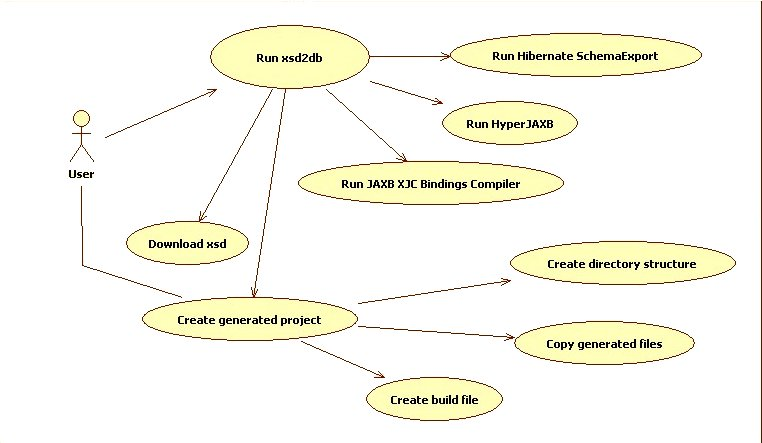
\includegraphics[scale=0.5]{./Images/xsd2dbUseCase.jpg}
\caption{Use case diagram for xsd2db}
\label{xsd2dbUMLUseCase}
\end{center}
\end{figure}

In order to download a schema file we did blah blah blah 
%scott can you fill this in if not I will come up with something.

To call the JAXB bindings compiler one must first create a com.sun.tools.xjc.Options object.  You must then use the Options object to set the target directory for generated JAXB object files, the schema type of theXMLschema (DTD or XSD), and finally the location of the schema to be parsed.  Once the Options object is configured you can annotate the schema and create a annotated grammar by invoking the com.sun.tools.xjc.GrammarLoader.load()  factory method on the Options object and an ErrorReceiver object.  An ErrorReceiver is simply an object that implements the com.sun.tools.XJC.ErrorReceiver interface and allows a developer to decided how to handle errors;  in our case we simply reported them to the command line.   Once you have created an annotated grammar the XJC bindings compiler can be invoked using the static method Driver.generateCode() method on the AnnotatedGrammer, XJC Options object, and the ErrorReciver.  Some sample code is shown in figure \ref{XJCsamplecode}.
\begin{figure}[htbp]
\begin{center}
\begin{verbatim}     
        ErrorReceiver errorReceiver = new ErrorReceiverImpl();
        AnnotatedGrammar grammar = null;
        try {
            // Create a annotated grammar
            grammar = GrammarLoader.load(XJCOptions, errorReceiver);
            if (grammar == null)
                System.out.println("Unable to parse schema");
        } catch(Exception e) {
            System.out.println("Error loading the grammar");
            e.printStackTrace(); 
        }
        try {
            // Generate the JAXB objects
            GeneratorContext generatorContext;
            generatorContext = Driver.generateCode(
                 grammar, 
                 XJCOptions, 
                 errorReceiver);
            if (generatorContext == null)
                System.out.println("failed to compile a schema");
          }
        
\end{verbatim}

\caption{Code to invoke the JAXB XJC bindings compiler.}
\label{XJCsamplecode}
\end{center}
\end{figure}

To invoke thehyperjaxb2add-on we take advantage of the fact that all JAXB add-ons must provide a run method since they implement the JAXB AbstractParameterizableCodeAugmenter interface.  Thus to create the hibernate mapping files for the generated JAXB objects, we create a new Hyperjaxb2 add-on and call run using the AnnotatedGrammar, GeneratorContext,  and XJC Options Objects that we created when invoking the XJC bindings compiler. 

In order to generate the SQL DDL file we use the Hibernate SchemaExport object.  Hibernate requires that Hibernate Configuration object be created and configured before any hibernate objects can be used.  To configure the Hibernate Configuration object we simply load an included Hibernate properties file and use the Hibernate Configuration object's setProperties method to configure Hibernate.  The last step of the Hibernate Configuration is to inform hibernate of the location of the hibernate mapping files that it will be using.  In \emph{xsd2db} we decided to do this manually using the Configuration object's addFile() method.   Once hibernate is configured generating a SQL DDL file is very simple.  All we must do is create a new SchemaExporter, set the output directory for the DDL file, set the delimiter for the DDL file, and finally create the DDL file by calling the create() method on the SchemaExporter.  Sample code can be seen in figure \ref{schemaExportSampleCode}.
\begin{figure}[htbp]
\begin{center}
\begin{verbatim}
         // Initialize hibernate
        hibernateConfig = new Configuration();
        File hibPropertiesFile = new File(HIB_PROPERTIES);
        Properties hibProperties = new Properties();
        try {
            hibProperties.load(new FileInputStream(hibPropertiesFile));
        } catch(Exception e) {
            System.out.println("Properties file failed to load.");
        }
        hibernateConfig.setProperties(hibProperties);

         // Add a hibernate mapping file
         hibernateConfig.addFile(hbmMappingFile);
         
        // Produce the SQL file.
        SchemaExport schemaExporter = new SchemaExport(hibernateConfig);
        schemaExporter.setOutputFile(fullOutputPath);
        schemaExporter.setDelimiter(";");
        schemaExporter.create(true, false);
\end{verbatim}
\caption{Schema export sample code}
\label{schemaExportSampleCode}
\end{center}
\end{figure}

The Last phase of \emph{xsd2db} is to create a standalone project that is ready to be compiled using ant.  To this end we first create a project directory structure. The structure produced is that shown in figure \ref{xsd2dbStructure}.  We then copied the necessary library files need to compile the generated project from the lib directory of \emph{xsd2db} to the lib directory of the generated project.  Finally we generate a build file using a canned build file that we included as a resource in the \emph{xsd2db} jar.   

\begin{figure}[htbp]
\begin{center}
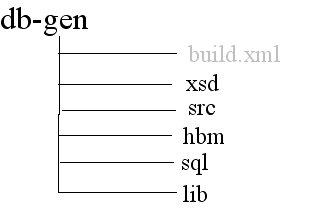
\includegraphics[scale=0.8]{./Images/xsd2dbStructure.jpg}
\caption{{\bf \emph{xsd2db}output project directory structure}}
\label{xsd2dbStructure}
\end{center}
\end{figure}

After this last phase the user can then compile the output of \emph{xsd2db} using the generated build file.  The resultant out put is a java library file that can be combined with the \emph{xmlpipedbutils} described in section \ref{xmlpipedbutils} to create a functional application capable of importing and querying data from the usersXMLsources to a relational database.

\subsubsection{Performance Analysis}
\emph{xsd2db} has been tested on three differentXMLschema files with varying degrees of success.  We preformed initial testing on the books.xsd schema.  Books.xsd is the canonical schema used in most example applications that useXMLdata and thus we felt it was an appropriate choice as our initial test schema.  When using \emph{xsd2db} we were able to importXMLdata into a Postgresql database, and later query that database without making any modifications to our generated files.  The success of this initial test lead us to try using \emph{xsd2db} on two other schemas: Uniprot.xsd and the GO DTD schema.  

After running \emph{xsd2db} on the Uniprot.xsd we discovered that some post processing would be required on the generated project before we would be able to importXMLdata into a Postgresql database.  This was largely due to several incompatiblities with the Postgresql database and no fault of \emph{xsd2db}.  However, one problem did arise which was a direct occurance of a failure of \emph{xsd2db} to properly handle XSD union types.  This was later attributed to a bug in \hyperjaxb2~  and remains a part of \emph{xsd2db}.  We created another tool, uniprotdb, to resolve these issues by post processing the output of \emph{xsd2db}.  A more thorough examination of these problems as well as a detailed description of uniprotdb can be found in section \ref{uniprotdb}.

The last schema file we tested \emph{xsd2db} on was the GO schema file.  The GO schema file presented a unique challenge in that it differed from the other schemas we tested \emph{xsd2db} on since it was DTD and not an XSD schema.  Again as with the Uniprot.xsd we encounter some problems with Postgresql and had to develop a post processor for GO, \emph{godb}.  \emph{godb} and the problems we encountered are described in more detail in section \ref{godb}.

In addition to the test we preformed with these three different schemas \emph{xsd2db} also contains several unit test of the command line interface.  Thus we are sure that the command line interface works and is bug free.

Overall it can be said, that \emph{xsd2db} does what is intended.  It is a metatool for developers to create there own xml import engines, thus it is reasonable that it might require post processing depending on a developer's design choices.  However, despite this initial success it is clear that there remains work to be done to improve the performance and robustness of \emph{xsd2db}. 

\subsubsection{Future Work}
For the first round of development we initially focused on simply getting \emph{xsd2db} working as quickly as possible.  While some minor unit testing has been preformed as well as a good amount of maintenance to re-factor the code base, more can always be done.  

One aspect we would like to work on would be to improve the compatibility of \emph{xsd2db} with the Postgresql database.  This would fix  the problems with both biological databases referenced in sections \ref{uniprotdb} and \ref{godb}.  In addition, on the same line of thought we would like to fix the XSD union bug in \hyperjaxb2.

Another area of improvement in \emph{xsd2db} would be to develop more unit test for both the \emph{xsd2db} command line and the \emph{xsd2db} functional unit.  When the unit test were initially written for xsd2db the functional component was not written in a state that would lend itself to be easily unit tested.  It has since been re-factored and unit test should be written.

The last area of improvement, would be to possibly add a graphical interface to \emph{xsd2db}.  While \emph{xsd2db} is primarily intended as a tool for developers and thus a command line interface is appropriate, adding a graphical interface to \emph{xsd2db} can only ease its use.





%Babak, David, Jeffrey%
\subsection{Performing Common Operations with \emph{xmlpipedbutils}}

%Jeffrey%
\subsection{Client Configuration}
In order to make the tools as easy to use as possible the issue of Hibernate properties configuration had to be addressed. Hibernate supports a wide variety of databases and data access methods. While advantageous for technical people, this can make configuration a daunting task for others. We choose an approach that would be modular, allowing the configuration component to be plugged into any application seamlessly. This was achieved by breaking the component in to four distinct objects: HibernateProperty, HibernatePropertiesModel, ConfigurationController and ConfigurationPanel. The ConfigurationController loads the structure of the Hibernate properties along with default values into a HibernatePropertiesModel. Each property is represented by a HibernateProperty object in the model. HibernateProperty objects consist of a category, type, name and value, as well as an indicator of whether the property is saved or not. This allows both saved and unsaved properties to be stored in the same model. The model is used by the ConfigurationPanel to render the a GUI for the user to view and/or edit the properties. When properties are saved, a model object is passed back to the controller, which then stores the properties in a hibernate.properties file.



%David%
\subsubsection{XML Import}


%Babak%
\subsubsection{Ad Hoc Queries}
A major factor in any research tool is data analysis. To this end, we are providing users of xmlpipedbutils with two query tools: an SQL analyzer and an HQL analyzer. Each of these views allows for a different view of the data and allows each user to utilize the query language they are most familiar with.

\paragraph{GUI Design}

The query panel is split into three sections; each separated by a splitter. On the left of the user interface is the query section. The radio and command buttons are on the right. The right side consists of two radio buttons and two buttons. The two buttons let the user choose between standard query language (SQL) and hibernate query language (HQL) queries. 

The left side is further split into two other sections. The north section contains a text area in which the query can be typed. The bottom of the panel contains two components: a table and a tree. How each view is populated depends on whether we are executing an SQL query versus an HQL query.

The command buttons are labeled ``Clear'' and ``Execute Query''. Clicking on clear will erase the text from the query text are and clear any data from the results table and tree. Clicking the execute button will execute the query in the text area and populate either the tree or the table with the returned data. We will discuss how the data is displayed further in the following sections.

\paragraph{SQL Analyzer}

The SQL Analyzer allows the user to execute SQL queries and view their results. The results of the query (if any) are displayed in a table in the user interface. The table's heading is updated to match the field names of the results.

The result table is a simple JTable. The DefaultTableModel object associated with the JTable allows for all manipulations of the table's data.

Each executed query returns a ResultSet object. The ResultSetMetaData object associated with the ResultSet instance provides the names for each of the returned columns. These column names are used for the table model's header. The table model is then populated one row at a time using the ResultSet.

\paragraph{HQL Analyzer}

The HQL analyzer works just like the SQL analyzer in that the user can manually type in any query, click the execute query button, and view the results. Where as the SQL analyzer would display all of the results in a table, the results from the HQL queries are displayed in an object tree. The tree displays each object's hierarchy within a tree structure.

The tree is implemented as a customized JTree. Each of the objects returned by the Hibernate query are stored as the user object of a DefaultMutableTreeNode. Each of the properties of the object for which we have a getter and/or setter are further represented as children of the nodes. This recursive deepening goes until we reach the core Java classes.

\paragraph{Usage}
Using the query analyzer is identical whether working with SQL or HQL. The query is entered in the text box on the north side of user interface. The radio buttons on the right allow the user to designate the entered query as either SQL or HQL. The results of an SQL query are displayed in a table format. Since and HQL query returns a set of objects, the results of an HQL query are displayed in an object tree in order to display the breakdown of each object.

\paragraph{Future Modifications}
We will now discuss some changes that are being considered for the next iteration of the utilities. The user interface and the object tree still have plenty of modifications that can be performed and these will be addressed in the near future.

1. Currently, the object tree is populated with all of the returned data upon executing the query. While this works fine for small sets of objects, this is not efficient for large data sets. For the next iteration we will maintain a copy of the returned objects locally, but we will only populate the first level of the tree. Each sub tree will be further populated as the user expands the corresponding tree nodes.

2. The user interface currently displays both the result table and the object tree simultaneously. The next update should display only one of these components at a time. Upon selecting each of the radio buttons designating which type of query we are working with, the proper component should be made visible. Selecting the SQL radio button shall display the result table and selecting the HQL radio button shall display the object tree.


%Joe, Joey, Roberto, Scott%
\section{Application to Biological Databases}
\label{biodb}
% First three paragraphs added by Joe Boyle 4/30/2006
% Need Scott or Roberto to add information about GO
The GenMAPP application uses a gene database that contains species-specific
libraries of gene information.  The database is needed in order to link expression
data with MAPPs, for creating and modifying MAPPs, and for importing new data.
The gene database contains two main types of tables, Gene Tables and Relationship
Tables.  A Gene table is a collection of gene identifiers obtained from a
cataloging system for a particular species.  A Relationship Table provides a link
between gene IDs of two separate gene ID databases.  These tables are essential to
the GenMAPP application~\cite{noSupport}.

GenMAPP gene databases function around a central system, known as the MOD system.
A Model Organism Database (MOD) is a public database that contains genes and
annotation for a particular organism.
The purpose of using a MOD system within GenMAPP is to form a link between
GenMAPP and the gene ontology (GO) hierarchy~\cite{noSupport}.  Current gene
databases supplied by GenMAPP use the Ensembl database to link to GO.  However,
Ensembl is limited to the number of species it represents, which is only
mammalian organisms.
As a result, for the XMLPipeDB project, UniProt was chosen to form the link to GO
based on the number of species available from it.  In this case, UniProt is not
actually a MOD in the strict sense of the word.  But it can be used to form the
needed link to the GO hierarchy.

UniProt (Universal Protein Resource) is the world's most comprehensive catalog of
information on proteins~\cite{uniprotWeb}.
The European Bioinformatics (EBI) group and the
Swiss Institute of Bioinformatics (SIB) produced Swiss-Prot and TrEMBL
(Translated EMBL Nucleotide Sequence Data Library)
whereas
Protein Information Resource (PIR) produced the Protein Sequence Database (PIR-PSD).
By noticing that the information contained in these separate databases was beginning
to overlap, the UniProt Consortium was formed.
UniProt has now become the central repository
for protein sequence and function after joining the information found in
Swiss-Prot, TrEMBL, and PIR databases.

% added by Scott Spicer 02-May-2006
The Gene Ontology database provides consistent descriptions of gene products present
in other public databases. The GO consortium is developing three structured, controlled
vocabularies (ontologies) that describe gene products in
terms of their associated biological processes, cellular components and molecular functions
in a species-independent manner. The GO table in the Gene Database stores the individual
GO terms and their relationship to each other. Since the GO ID does not refer to a gene,
it is not an appropriate gene ID system to use as primary ID on a MAPP 
(a special file format produced by GenMAPP) or in a Gene Expression Dataset~\cite{genmapp.com}.


%Joe, Joey%
\subsection{UniProt}
\label{uniprotdb}

\subsubsection{Introduction}
It is important to restate the goal of the \xmlpipedb~project before understanding 
the important role \emph{uniprotdb} played in the project; To create a reusable tool set 
that given genomic sequencing data for an organism in XML and a schema for that 
XML document could output a working \genmapp~gene database for that organism.  During
the beginning phases of the project, there was only one project, \xmlpipedb, and it
made use of the schema provided by the UniProt Consortium~\cite{uniprotWeb}.  However,
it soon became evident that the project could be designed in a manner that would 
allow a wider audience the use of our tool.  The first phase was \emph{xsd2db} (Section~\ref{xsd2db})  which allowed for the use of any schema
to create the necessary JAXB objects and hibernate mappings.  However, we still
needed to create a tool specific for the UniProt XML and XSD.  At that point, \emph{uniprotdb}
was born.  

\subsubsection{Design}
Before the project was split into a variety of subprojects, \xmlpipedb~offered
the ability to use the UniProt schema and create the necessary JAXB objects
and \hibernate~mappings.  It created these files in default directories that 
are called out in the \hyperjaxb2~template project~\cite{hyperjaxb}.  Customizations were used in order to get \xmlpipedb~to work properly, but we hoped 
to further understand how to use \hyperjaxb2~customizations to overcome these issues.  
Section~\ref{uniprotImplementation} discusses in further detail the \hyperjaxb2~customizations that were needed for \xmlpipedb~to function.  

Once it was determined that we wanted to allow groups outside the Bioinformatics community the 
use of our tool, \emph{uniprotdb} became its own subproject.  \emph{uniprotdb}
would be created from the output of \emph{xsd2db}.  It would contain the UniProt schema,
customized external binding file, 
SQL DDL file that corresponds to the schema, the JAXB objects, and the \hibernate~mappings.  
The layout 
shown in Figure~\ref{fig:uniprotLayout} was what we hoped uniprotdb would look like.  

\begin{figure}[htp]
\centering
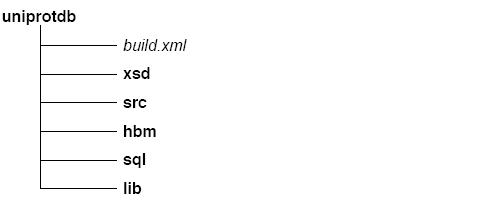
\includegraphics[scale=1.0]{Images/uniprotLayout.jpg}
\caption{\small \sl The uniprotdb layout.} 
\label{fig:uniprotLayout}
\end{figure}

The build file would have the following capabilities:
\begin{itemize}
  \item \textit{compile} compiles the JAXB objects located within the src directory with help from any necessary jars located in the lib directory

  \item \textit{jar} compile and create a jar file containing the class files derived from the src directory and the hibernate mappings located within the hbm directory
  
  \item \textit{clean} eliminates all the products of a previous build.  
\end{itemize}
The jar file created as a result of a build would later be used in the gmbuilder 
subproject, thoroughly outlined in Section~\ref{gmbuilder}.  Once uniprotdb was
created, we would have been one step closer to creating a \genmapp~usable, gene 
database.  

\subsubsection{Implementation}
\label{uniprotImplementation}
% discuss phases of the post processor and the failed usage of hibernate bindings
The work we did on the original \xmlpipedb~project set the stage for the creation of
uniprotdb.  
The work on the original \xmlpipedb~project brought us to a point where we were able to load
the SQL DDL file that was produced from the UniProt schema.  In addition, we were able to 
import the JAXB objects into the database.  Before this point was reached though, we had to
overcome three issues with the hyperjaxb2 and the UniProt schema.  The issues that slowed our 
progress with \xmlpipedb~were:
\begin{itemize}
   \item PostgreSQL doesn�t like attributes whose name is ``end'' (see LocationType in UniProt XSD)
   
   \item String types default to a maximum length of 255 (varchar(255)), but some strings in the UniProt XML files exceed this length
   
   \item Hyperjaxb2's handling of the xsd:union tag doesn�t seem to work properly, resulting in MappingExceptions when attempting to load an XML file
\end{itemize}

The solution at the time was to manually edit the generated files.  The
SQL DDL file that corresponds to the UniProt schema had a need for multiple edits.  The
first was to change``end'' to 
``endPosition.''  This solved the problem with keyword ``end'' in PostgreSQL.  
The second edit was to change ``varchar(255)'' to just ``varchar.''  This solved any issues with
there being a maximum length for strings within a UniProt XML file.  

Since we changed the SQL DDL column named ``end'' to 
``endPosition,'' the same change needed to be made to the corresponding hibernate mapping file.  
This edit took place within LocationType.hbm.xml.    
Lastly, CitationType.hbm.xml needed to be manually edited due to the xsd:union 
tag being an issue with hyperjaxb2.  The ``Date'' field of CitationType allowed for any form of Date,
whereas the best solution was to only allow strings.  So CitationType.hbm.xml was updated to only allow
strings for Citation Dates.  Once all these issues were resolved, the import of a UniProt XML file
into the database was no longer a problem.  

At about the time \xmlpipedb~was beginning to show promise, the decision was made to split the \xmlpipedb~project into a group of smaller projects that would allow for groups outside the Bioinformatics
community to use our tool.  Hence, uniprotdb was supposed to be a subproject specific to the 
UniProt schema.  Rather than forcing the user have to manually edit the output of xsd2db due to the issues
above, we looked
at the use of a customizable binding file within hyperjaxb2.  Custom binding files would allow for changes
to a schema and its generated files without any extra work required by the user.  The use of custom bindings 
files were looked at for a few weeks before it was stopped due to complexity and time constraints.  Refer to 
Section~\ref{uniprotImprovements} for further detail regarding custom bindings files.  

Once it was determined that custom bindings would not be used, we needed an alternative method to the 
editing of the generated files from xsd2db.  We decided to develop a post processor.  The post processor
would reside within the uniprotdb project under a new directory named tools.  Within the tools directory
would be a build file, a README file, and the necessary source code to do the post processing.  The build
file had the ability to compile the source code and eliminate all the products of a previous build.  

The post processor had the ability to be run via command line with options to specify the locations of the files
to be edited or with the use of a graphical user interface (GUI).  With the GUI, there are two windows shown
for each file.  The first window asks for the user to locate the file to post process.  It is shown in 
Figure~\ref{fig:locateFile}.  
\begin{figure}[htp]
\centering
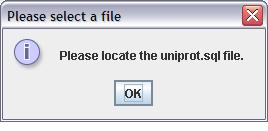
\includegraphics[scale=1.0]{Images/locateFile.jpg}
\caption{\small \sl The locate file dialog.} 
\label{fig:locateFile}
\end{figure}
Once the user hits the OK button, a second window appears.  The second window is a file dialog for the 
user to use as a navigator for the file to be processed.  It is shown in Figure~\ref{fig:chooseFile}.  
\begin{figure}[htp]
\centering
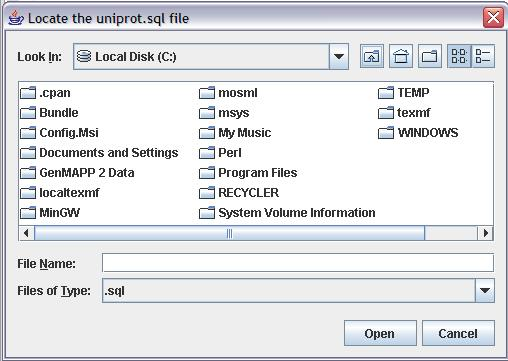
\includegraphics[scale=0.80]{Images/chooseFile.jpg}
\caption{\small \sl The choose file dialog.} 
\label{fig:chooseFile}
\end{figure}
After the last file is processed, the window in Figure~\ref{fig:success} appears to let the user know that 
the operation was successful.  
\begin{figure}[htp]
\centering
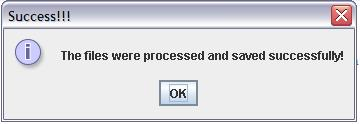
\includegraphics[scale=1.0]{Images/success.jpg}
\caption{\small \sl The success window.} 
\label{fig:success}
\end{figure}

Further testing resulted in the finding of more bugs with the ``Date'' field
in the schema.  As a result, the post processor needed to be updated to
process two more java classes.  CitationType.java and CitationTypeImpl.java both
needed post processing to make sure that the ``Date'' field used by the
JAXB objects would only return a object of type string.  With the addition
of two more files being post processed, the decision was made to no longer
make the command line version of the post processor available.  We felt
that the user should not be burdened with having to fill in the absolute
path for a total of five files.  

\subsubsection{Future Work and Improvements}
\label{uniprotImprovements}
The only visible improvement to uniprotdb would be to use a custom mapping file rather than a post 
processing tool.  The custom mapping file would be used with xsd2db and the UniProt schema and would
allow custom mappings to be generated for classes and fields by annotating the schema.  This would no 
longer make a post processor needed.  

The future of uniprotdb is up in the air.  Only a small subset of the total UniProt XML files available 
have been imported into a database with gmbuilder.  
This means that more post processing may be needed because all the post processing
needs may have not been discovered.  As testing continues, the Bioinformatics community will need
to feel free to report any bugs and errors.  In addition, a new UniProt schema could become
available resulting in more post processing.  As a result, it will be the responsibility of 
this group of developers to keep track of the ever changing Bioinformatics landscape.  

\subsubsection{Conclusion}
uniprotdb is important in order to reach our goal of creating a gene database that can be used by
the \genmapp~application.  xsd2db creates the necessary JAXB objects and hibernate mappings corresponding
to the UniProt schema.  The uniprotdb post processing tool also appears to work with the current
UniProt schema.  However, a much cleaner implementation would make use of a custom bindings file.  Future
implementations of uniprotdb should look at the process of creating custom bindings file again.  
It must be noted though, as simple as uniprotdb is, it is crucial for gmbuilder application 
to function properly.  


%Roberto, Scott%
%\documentclass[12pt]{article}
%\begin{document}


\subsection{Gene Ontology}
% Updated by Roberto and Scott
The Gene Ontology (henceforth GO) database is a staging database created to hold the records describing gene products according to biological processes,
cellular component, and molecular functions. This database allows the user to extract structured-controlled vocabulary terms
which describe gene products in any organism~\cite{geneontologyWeb}. In particular, Escherichia coli related data is queried as a part of the main
objective of the xmlpipedb project.

\subsubsection{Introduction}
GO and Uniprot, which is described in Section~\ref{uniprotdb}, are the two data strucures needed to output a
working GenMAPP gene database for a partiuclar organism. During the beginning phases of the original XMLPipeDB project,
only Uniprot had been included into the build process; GO came along after the project was broken into subprojects,
which was named godb. The first step in creating a godb deliverable was to run a GO schema file
through xsd2db, which is described in Section~\ref{xsd2db}. xsd2db generates the necessary JAXB
objects, hibernate mappings, SQL DDL file, and the godb build file. The build file is then executed
to produce a deliverable jar file which  would later be used in the gmbuilder
subproject, which is described in Section~\ref{gmbuilder}.


\subsubsection{Design}
\label{godtd}
GO exports its data to a number of different file formats to allow flexibility for different users with
different background and purposes. For this subproject, choosing a file format proved to be a difficult task.
There are three main file formats to extract GO data: flat files, mySQL formats, and XML files. Flat files
were eliminate because they are not compatible with JAXB classes (Java Architecture for XML Binding), which  are called by
xmlpipedb utilities. MySQL format were eliminated because a ``one-off" tool would need
to be created to port the data from mySQL to postgres. Initially, this format was considered since xsd2db
required a XSD
schema file (hence its name), which GO did not provide. A later version of xsd2db supported DTD schemas, which GO uses to define their
schema definitions. If we used mySQL, then what happens if the schema changes? The ``one-off" tool would need to be changed every
time GO changed its schema, which would be costly and inefficient. But xsd2db provides the ability to auto generate any time GO changes
their schema, so the mySQL format was not passed on, which left XML formats.

GO provides their data in two XML format which both contain DTD schema files: OBO.xml and RDF.xml. However,
the members of the GO Consortium claimed that they will eventually generate a XSD schema for OBO.xml, and that there
are no plans to generate an XSD schema for the RDF file. In fact, they only reason why they currently have a DTD file
for RDF.xml is for historical reasons. Thus, the OBO.xml file format
was chosen for the project, and therefore the OBO.dtd file was fed into xsd2db.

As it turned out, the OBO.dtd file produced a SQL schema that contained a tabled name \emph{To}, which happens to be
a postgresSQL keyword. Furthermore, since the DTD file did not specify a maximum character length for all GO tags-value
pairs, the SQL schema defaulted those tags to type \emph{varchar(255)}. Unfortunately, though, some of the data exceeds the
character limit of 255. Due to the variety of problems, a godb postprocessor was created.

\subsubsection{Postprocessor}
The godb postprocessor is a GUI based tool to fix the errors in section~\ref{godtd}. Two files needed to be modified  before
godb can be delivered: \emph{schema.sql} and \emph{To.hbm.xml}. For the \emph{schema.sql} file, the postprocessor
searched and replaced all instances of \emph{varchar(255)} to \emph{varchar}, which specifies an unlimited character string type.
Thus, any data that exceeded 255 characters would not generate an error. Additionally,
the postprocessor changed the table name \emph{To} to  \emph{To\_}, which eliminates any conflicts with postgresSQL keywords.
Xsd2db, however,
creates a xml hibernate mapping file that expects there to be a table named \emph{To}, which moves us on to the second file to modify,
\emph{To.hbm.xml}. Within this XML file, there is an \emph{table} element that defines the table name for this mapping, which had the
value of \emph{To}. Thus, the postprocessor simply replaced this value from \emph{To} to \emph{To\_}.

In the interest of flexibility, the postprocessor GUI asks the user to supply the file names to be modified.
Once each file has been selected, the tools proceeds to fix the corresponding files and returns a success message
if the changes were done correctly, otherwise the application terminates without modifying the files.

\subsubsection{Performance Analysis}
Once the godb ran through the postprocessor, a OBO.xml was loaded using the import features of xmlpipedb utilities.
Unfortunately, the import failed; fortunately it was simply a memory heap issue: since the OBO.xml file contains alot of data, and
JaxB instantiates the ``entire" object graph in memory before committing it to the database, an \emph{out of memory} error was issue.
To fix this, the java \emph{maximum heap size} was increased to 1024mb, and the subsequent import was successful. It took
around 40 minutes to load the entire file on a 2.0GHz machine.

The godb served its purpose because all the data from gene ontology was successfully uploaded.  The database access was also
successfully executed by gmbuilder without any major problems.  The development of this part of the project was facilitated
in part because the uniprot database.  The functionality of the postprocessor was mirrored from the same postprocessor
developed by uniprot db.  By using the same code design as the uniprot postprocessor, the future maintenance of the godb
code can be done in parallel with any changes done on the uniprot db side.

\subsubsection{Future Work}
The future work with the godb can be extensive.  However, in order to have a good understanding of
future change requests, the developers must work together with biologists to find relevant information needed to support their requests.
After all, the biologist are the end users. One potential issue with  godb is that it was only tested on a postgres database. In other
words, other databases may require additional/other fixes to be performed by the postprocessor. If that were the case, then
the postprocessor tool would need to change to allow the user to select the database type. Integration test would also have to be performed
in using another database.

Another future work that can be done is
documentation.  Although the godb project successfully performed its work, it was not documented properly.  A software
requirement specification can be prepared which lists all the requirements on the database and the postprocessor tool.  The
delivery of this document can give an idea to users and developers on how to proceed when using or modifying the godb
applications.

%\end{document}


%Joey%
\subsection{GenMAPP Builder}
\label{gmbuilder}

\subsubsection{Introduction}
GenMAPP Builder is a GUI application for loading, querying, and exporting data
used by GenMAPP.

\subsubsection{Design}

GenMAPP Builder is also tasked to export GO data from postgres to a Microsoft Access (MDB) file.
GenMAPP requires four GO tables to be populated with data: GeneOntology,
GeneOntologyTree, GeneOntologyCount, and Uniprot-GeneOntology. At runtime, each table
is created in the MDB file prior data is inserted. 
The following sections will discuss each table.

\paragraph{GeneOntology}
\label{gotable}
The GeneOntology table consists of a list of GO terms, which is created by extracting all the
GO terms from the postgres database by executing HQL statements. Each term has required tags, \emph{Id} and \emph{Name}.
Each term may contain optional tags, one of which is an \emph{is\_a} tag. An \emph{is\_a} tag describes a
subclassing relationship between one term and another. Since GO terms
are organized in structures called directed acyclic graphs (DAG), each term may have many \emph{is\_a} relationships.
Terms with no \emph{is\_a} relationships are roots. Each term represents an entry in the GeneOntology table. If a term
has no \emph{is\_a} relationships, then one row is inserted into the table. If a term has one or more
\emph{is\_a} relationships, a row is inserted for each \emph{is\_a} relationships using the same term Id.


\paragraph{GeneOntologyTree}
The GeneOntologyTree table contains a tree representation of the GO DAG structure, which is used by MAPPFinder
to build the GO tree in the MAPPFinder browser. The algorithm that creates this table starts by inserting the root
node for each ontology. After inserting the root node, it then grabs all the children of that node and perform an insert.
For each child, it grabs its children
and performs an insert. This process continues recursively, and stops when no more child nodes exist.
Unfortunately, this table is not created from postgres, but rather from the
newly created table in Section~\ref{gotable}. The OBO.dtd file creates a SQL DDL schema which does not support
the ability to extract child nodes from a parent node. The GeneOntology table provides this functionality, which
is why it must be created first. Thus, the algorithm actually queries the MDB Access file using SQL statements.


\paragraph{GeneOntologyCount}
The GeneOntologyCount table contains the of number of times a GO ID appears in the GeneOntologyTree table, which
is also used by MAPPFinder to build the GO tree in the MAPPFinder browser. During the creating of the GeneOntologyTree
table, a count of each GO ID is stored in a data structure. In other words, when the algorithm grabs all child nodes from
a parent, each child node's count is increment by 1. When the GeneOntologyTree table is complete, the count for
each GO ID is extracted from the data structure and inserted into the GeneOntologyCount table.
This method was used to ``kill two birds with one stone". Otherwise,
the algorithm would have to wait until the GeneOntologyTree table was complete. Then for each GO ID, the algorithm would have
to query the GeneOntologyTree to extract the number of times it showed up in the table, which is costly and inefficient.


\paragraph{Uniprot-GeneOntology}
The Uniprot-GeneOntology table provides a mapping between a Uniprot ID and a GO ID, which is a many to many relationship.
Currently this information is not found in godb, but rather in a associations text file which is part of the GenMAPP Builder
resource library. Each line in the text file may contain a Uniprot ID. If it does, then there will be one to many GO ID's.
Thus, for each GO ID, a new row is created in the Uniprot-GeneOntology table with the Uniprot ID as one field and the GO ID
as another field. For example, if the line contained a Uniprot ID of \emph{00001} and three GO ID's \emph{10001,10002, and 10003},
then three row would be created with values ``00001 10001", ``00001 10002", and ``00001 10003."

\subsubsection{Performance Analysis}
A couple of GO errors occurred during the first run of gmbuilder: two table fields are named \emph{Primary} and \emph{Level}, which
Microsoft Access interpreted as keywords. Additionally, the hyphen in the table \emph{Uniprot-GeneOntology}
was recognized  as a continuation line, and therefore a syntax error was generated. Fortunately, the same fix was used
in all three cases: enclose each name in double quotes. After the fix was implemented, gmbuilder successfully built the
GO tables in the MDB file, which took considerable time.

The time to build the four GO tables ran in the neighborhood of five hours (2.0GHz single processor), and
granted, this time can be shorten with better hardware. A big chunk of that time falls on the creation of the
GeneOntologyTree, although this table contains roughly seven time more entries than the table with the second
most entries. Still, it seemed that the rate of insertions per second was larger.
A good test would be to time, call it T, the creation of the
GeneOntology table by itself, than take the number of entries that were created and divide it by T. Then do the same for the
GeneOntologyTree, and compare the rate of insertions per second. If they are approximately the same, then the increased time
is due to the increase in entries. But, if the GeneOntologyTree insertion rate was much higher, than further investigation would be
needed to why the rate is slower. Perhaps it's due to the recursive nature of the algorithm, since recursion increases overhead.


\subsubsection{Future Work}
Regarding the GO tables, the algorithm that populates the GeneOntologyTree table should be investigated.
If it turns out that the GeneOntologyTree insertion rate in considerable larger that the other tables, then
a couple of solutions can be analyzed: 1) create an equivalent non-recursive function to build the tree. This
eliminates the added overhead of recursion; 2) the code can be cleaned up to
close \emph{Statement} objects before the next call to the recursive function is made. Also, the code can
be modified to use \emph{PreparedStatement} object as opposed to \emph{Statement} objects, which may be more
efficient according the java API.


As of right now, Uniprot-GeneOntology associations file is defined at a specific location in the build tree,
and the code reflects that by hardcoding the path to the file. This is error prone: every time the file changes location,
the code would also have to change, which supports poor coding practices. Also, what is the user wanted to use a different
associations file? Then the file would have to be checked in as a new resource file, and a new version of the software would have
to be released. The solution is to make this file user selectable from the genMAPP Builder GUI. This eliminate the two problems
above, while add flexibility to the user.



\section{Conclusion}
Despite the pitfalls encountered, incredibly tight timeframes and demands of assimilating an entirely new domain of knowledge, the XmlPipeDb team has produced an initial release of outstanding quality and utility. In each area, we have identified additional work to be done, whether to add polish, tweak bugs or add new functionality. The real test will come, however, when the biological community begins to use the tool chain and reap the rewards of our effort. Our since hope is that it will meet their needs and allow them to make more interesting discoveries about the building blocks of life. Of course, there will be issues and we will rise to meet the challenge. There will also be additional databases to support and format changes. These, too, we will strive to accomodate. Of course, one of the great advantages of this tool chain being open source is that it is not left only to us to do this work, but to anyone with the vision and the will to make it happen.



\pagebreak
\bibliography{../xmlpipedb-refs}
\bibliographystyle{alpha}

\end{document}
